\section{Individual Models} \label{sec:individual}

In this section, we describe and evaluate individual word alignment models. All of the newly introduced models make use of the fact that NMT systems can be viewed as language models. 


\subsection{Baseline Models} \label{subsec:baseline_models}

The first model is \fastalign{} (MF). The second is attention-based soft word alignment extracted from MarianNMT (MM), which was trained without guided alignment.

For the rest, we will focus on models generating alignment scores (an unbounded real number corresponding to the quality of a possible alignment between two tokens) and not the alignments themselves.

\subsubsection*{One Token Translation ($M_1$)}

The simplest approach to get alignment scores is to compute translation probabilities using the MT (function $m$): $\forall s_i\in S, t_j \in T: p(s_i, t_j) = m(\{s_i\}, \{t_j\})$. Since MarianNMT outputs log probabilities, the values themselves have to be put through an exponential function. This approach requires $\sum_{s\in S} \sum_{t\in T} 1$ translation inferences for a single sentence.

\subsubsection*{Source Token Dropout ($M_2$)}

More refined approach was chosen by \citet{zintgraf2017visualizing} in which the alignment score is computed as the difference in target token probability when the source token is unknown. The exact approach is too computationally demanding (requires inferences with large amounts of replacement words), and therefore we use much simpler, yet conceptually similar, method.

Assume $m_j(S, T)$ produces the log probability of the $j$-th target token. The sentence $S^{M_2}_i$ can be defined in two ways:
\begin{gather*}
    \forall s_i \in S, t_j \in p(s_i, t_j) = m_j(S, t) - m_j(S^{a/b}_i , t_j)
\end{gather*}

\vspace{-0.8cm}

\begin{align*}
    & \text{Word deletion} M_2^a \\ 
    & S^{a}_i = s_0, s_1, \ldots, s_{i-1}, s_{i+1}, \ldots, s_{|S|} \\
    & \text{Word substitution} M_2^b \\ 
    & S^{b}_i = s_0, s_1, \ldots, s_{i-1}, \texttt{<unk>}, s_{i+1}, \ldots, s_{|S|}
\end{align*}

This requires $\sum_{s\in S} |T|$ token translation inferences, which is comparable to $M_1$.\footnote{The actual running time would be different, because in this case it is $|S|$ inferences of length $|T|$, while in $M_1$ it is $|S|\times|T|$ inferences of length $1$.}

\subsubsection*{Source and Target Dropout ($M_3$)}

A very similar method would be to also dropout the target token and examine how the sentence probability changes. Applying the two different ways of dropout leads to four versions of this approach. Note that in this case we compute the sentence probability (because the target word is hidden) and also do not subtract from the base sentence probability, but rather use the new sentence probability as it is. This probability should be the highest if the corresponding tokens are both obscured. 
\begin{gather*}
    \forall s_i \in S, t_j \in p(s_i, t_j) = m(S^{a/b}_i , T^{a/b}_j)
\end{gather*}

\vspace{-0.8cm}

\begin{align*}
    T^a_j &= t_0, t_1, \ldots, t_{j-1}, t_{j+1}, \ldots, t_{|T|} \\
    T^b_j &= t_0, t_1, \ldots, t_{j-1}, \texttt{<unk>}, t_{j+1}, \ldots, t_{|T|}
\end{align*}

\vspace{-0.8cm}

\begin{align*}
    & \text{Word deletion, deletion ($M_3^{aa}$)} & S^a_i, T^a_j \\
    & \text{Word deletion, substitution ($M_3^{ab}$)} & S^a_i, T^b_j \\
    & \text{Word substitution, deletion ($M_3^{ba}$)} & S^b_i, T^a_j \\
    & \text{Word substitution, substitution ($M_3^{bb}$)} & S^b_i, T^b_j
\end{align*}

This approach requires $\sum_{s\in S} \sum_{t\in T} |T_t^{a/b}|$ translation inferences, which is roughly $|T|$ times more than in $M_1$ and $M_2$, making it the most computationally demanding approach.

\subsubsection*{Symmetrization}

So far, we assumed that we only have access to a one-directional MT. In most scenarios, however, bi-directional (usually in the form of two separate MTs) systems are available. It is then also possible to get alignment $A'$ from target to source.

Having access to both $A$ and $A'$, it is then possible to create a new alignment $B$ with either higher precision through intersection or higher recall through union \citep{koehn2009statistical}.
\begin{gather*}
    X^T := \{(b, a): (a, b) \in X\} \\
    B_{prec} = A \cap A'^T \qquad B_{rec} = A \cup A'^T
\end{gather*}

We can make use of the fact that the models output alignment scores and create new alignment scores in the following way. This allows us to fine-tune the relevance of each of the directions as well as their combination. It does not, however, have the same effects as the union or the intersection, because it does not affect the number of aligned tokens.
\begin{gather*}
    \beta_0 \cdot p(s, t) + \beta_1 \cdot p^r(t, s) + \beta_2 \cdot p(s, t) \cdot p^r(t, s)
\end{gather*}

\subsection{Direct Alignment from Baseline Models}

All of the models (except for \fastalign{}) are not producing the alignments themselves, but an alignments score $p$ for each pair of tokens $(s, t)$ in source $S$ $\times$ target $T$ sentence. The hard alignment itself can then be computed in the following ways. The parameter $\alpha$ can be estimated from the development set.

\begin{enumerate}
    \item For every source token $s$ take the target tokens $t$ with the maximum score.
    \begin{gather*}
        A_1^\alpha = \bigcup_{s \in S} \{ (s, t): p(s,t) = max_{t'} \{p(s,t') \} \}
    \end{gather*}
    
    \item For every source token $s$ take all target tokens $t$ with high enough score.
    \begin{gather*}
        A_2^\alpha = \bigcup_{s \in S} \{(s, t): p(s,t) \ge \alpha \}
    \end{gather*}
    
    \item For every source token $s$ take any target token which has a score of at least $\alpha$ times the score of the best candidate. This requires special handling for negative cases.
    \begin{gather*}
        A_3^\alpha = \bigcup_{s \in S} \{ (s, t): p(s,t) \ge min \\
        \big[ argmax_t\ p(s,t) \cdot \alpha, argmax_t\ p(s,t) / \alpha \big] \}
    \end{gather*}
    $A_1$ can then be expressed as $A_3^1$. Lower $alpha$ values lead to lower precision and higher recall because the algorithm includes more, less probable, alignments.
    
    \item Similar approach for $A_3$, but with the focus on the target side. For every target token $t$ take any source token which has a score of at least $\alpha$ times the score of the best candidate.
    \begin{gather*}
        A_4^\alpha = \bigcup_{s \in S} \{ (s, t): p(s,t) \ge min \\
        \big[ argmax_r\ p(r,t) \cdot \alpha, argmax_r\ p(r,t) / \alpha \big] \}
    \end{gather*}
    Similar reversal for $A_2$ would not make sense, because it takes all alignment above a threshold without any consideration for the direction.
\end{enumerate}

An exception to this would be modified $M_3$ approach, in which instead of having a single dropout on the target side, there could be multiple of them. This way, the score would not be between the source token and the target token, but between the source token and a subset of all of the target tokens. This would, however, lead to exponential complexity in terms of target sentence length. The dropout count would then have to be limited to the number of alignments to a single token that we can empirically expect of the given language pair. \Cref{fig:alignment_example} suggests that for English-German this could be 3.

\subsubsection*{Coverage}

The suggested greedy way of computing alignments from alignment scores is far from perfect. Imagine the following scenario depicted in \Cref{fig:alignment_coverage}, where the tokens C, D, and E have already been paired with a token A. The token F should then be more inclined to align with token B, which is, however, not modelled by the suggested approach.

\begin{figure}[h!]
    \center
    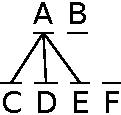
\includegraphics[width=0.11\textwidth]{img/alignment_coverage.pdf}
    \caption{
        Example of an alignment in which both B and F have not yet been paired with other tokens, but the greedy alignment approach does not take this into consideration.
        \label{fig:alignment_coverage}
    }
\end{figure}

\section{Evaluation of Individual Models}

\paragraph{Baseline Models} \Cref{fig:individual_encs_mix_a2} shows the results on Czech$\leftrightarrow$English data (averaged from both directions). Different models have different spans of their scores, and therefore it is much harder to select the single best $\alpha$. The most basic model, $M_1$, achieves the best results ($F_1 = 0.54$). The figure serves as an illustration of the $A_2^\alpha$ landscape.

\begin{figure*}[h!]
    \center
    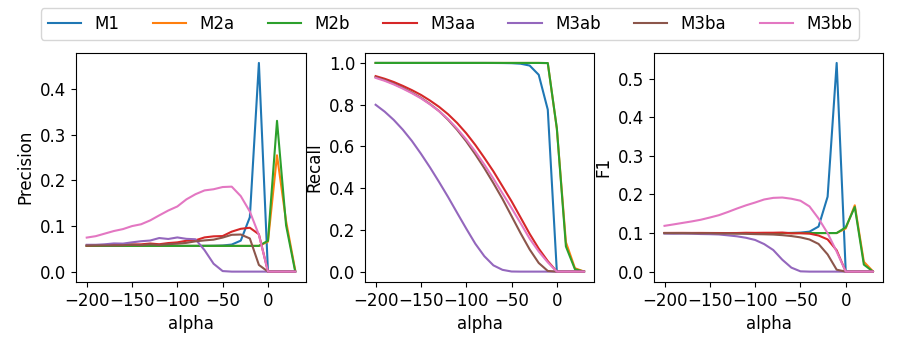
\includegraphics[width=0.8\textwidth]{img/individual_encs_mix_a2.png}
    \caption{Precision, Recall and F1 scores of individual models on averaged CS$\leftrightarrow$EN data extracted using $A_2$ \label{fig:individual_encs_mix_a2}}
\end{figure*}

The results on Czech$\leftrightarrow$English data (averaged from both directions) can be seen in \Cref{fig:individual_encs_mix_a3}. $\alpha = 0$ corresponds to predicting everything, while $\alpha = 1$ means predicting only the token with the highest score. The different model families behave similarly with respect to Precision, Recall and F1 score. $M_1$ achieves again the best results ($F_1 = 0.66$), but with the distinction between models being now more smooth.

\begin{figure*}[h!]
    \center
    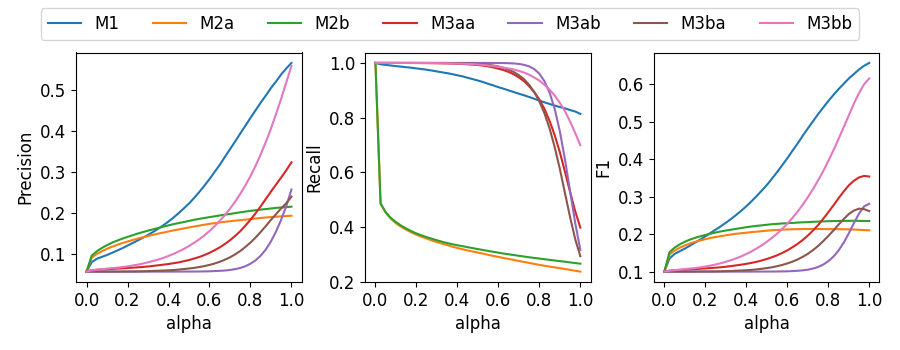
\includegraphics[width=0.8\textwidth]{img/individual_encs_mix_a3.png}
    \caption{Precision, Recall and $F_1$ scores of individual models on averaged CS$\leftrightarrow$EN data extracted using $A_3$ \label{fig:individual_encs_mix_a3}}
\end{figure*}

Interestingly enough, in \Cref{fig:individual_encs_mix_a2} out of the model $M_3$ family, only $M_3^{bb}$ showed to be successful more than the average. The other models, $M_3^{aa}$, $M_3^{ab}$ and $M_3^{ba}$, perform worse than $M_2^a$ and $M_2^b$. This is reversed by using the $A_3$ extractor, as shown in \Cref{fig:individual_encs_mix_a2}. For the $M_3$ model family, models with mixed obscuring functions ($M_3^{ab}$ and $M_3^{ba}$) perform worse than with the same function on both the source and target side ($M_3^{aa}$ and $M_3^{bb}$).

The English$\rightarrow$German dataset proved to be more difficult to process. The results, shown in \Cref{fig:individual_ende_a3}, are lower than for Czech$\leftrightarrow$English. The model $M_1$ again achieves the best results with $F_1 = 0.57$. The model ordering is however preserved from \Cref{fig:individual_encs_mix_a3}.

\begin{figure*}[h!]
    \center
    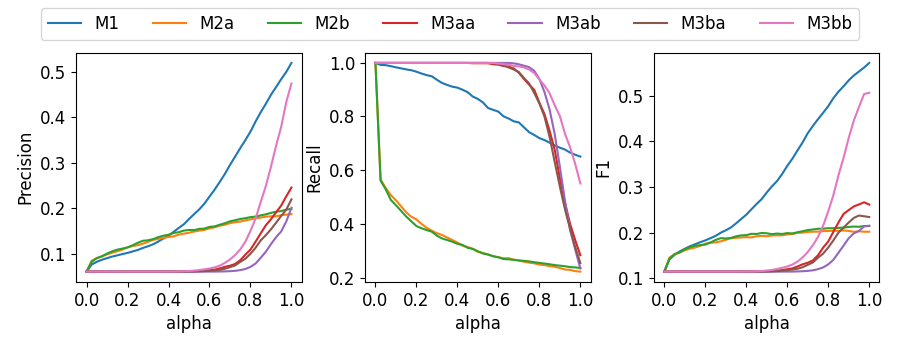
\includegraphics[width=0.8\textwidth]{img/individual_ende_a3.png}
    \caption{Precision, Recall and $F_1$ scores of individual models on EN$\rightarrow$DE data extracted using $A_3$ \label{fig:individual_ende_a3}}
\end{figure*}

\Cref{fig:individual_ts_encs_mix_a3} documents that different model types produce different number of alignments per one token. It also shows that the performance rapidly decreases with sentence length. The low results in \Cref{fig:individual_encs_mix_a3} can be explained by the dataset containing mostly longer sentences (21 tokens on average). The model $M_1$ is still better than $M_3^{bb}$ even on longer sentences despite the fact it does not model the context at all.
From both cases, we can see that $A_3^1 = A_1$ appears to be the best extractor for individual baseline models.

The best results were achieved with $A_4^1$ using $M_1$: $F_1 = 0.70$ for German$\rightarrow$English and $F_1 = 0.68$ for Czech$\leftrightarrow$English. The plots are very similar to those of $A_3$. Hence $M_3^{bb}$ follows up with $F_1 = 0.62$ and $F_1 = 0.64$ for German and Czech respectively.  

\begin{figure*}[h!]
    \center
    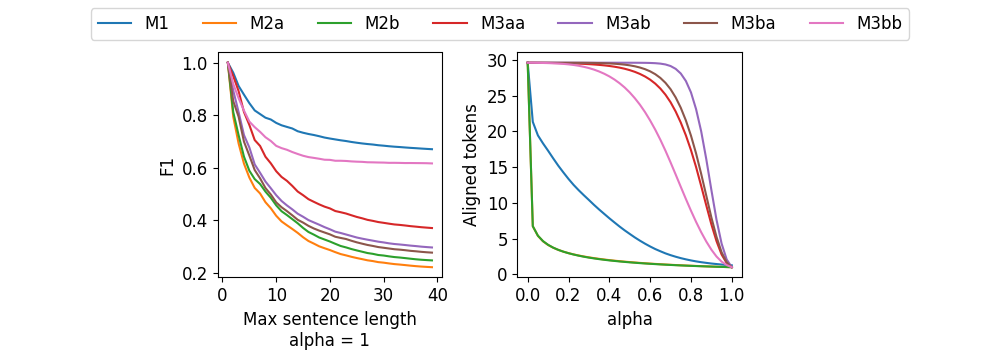
\includegraphics[width=0.89\textwidth]{img/individual_ts_encs_mix_a3.png}
    \caption{$F_1$ for $\alpha=1$ (left) and average number of aligned tokens (right) of individual baseline models on averaged CS$\leftrightarrow$EN data extracted using $A_3$ \label{fig:individual_ts_encs_mix_a3}}
\end{figure*}

\begin{table*}[h!]
    \center
    \begin{tabular}{lccc}
        \toprule
        Data & Precision & Recall & F1 \\
        \midrule
        Czech$\leftrightarrow$English & $0.54$ & $0.66$ & $0.59$ \\
        German$\rightarrow$English Small & $0.49$ & $0.55$ & $0.51$\\
        German$\rightarrow$English Small+Big & $0.62$ & $0.72$ & $0.66$ \\
        \bottomrule
    \end{tabular}
    \caption{Precision, Recall and $F_1$ scores of \fastalign{}. German$\rightarrow$English Small+Big was evaluated only on the annotated part. \label{tab:individual_fastalign}}
\end{table*}

\paragraph{\fastalign{}} In comparison, the results of \fastalign{} can be seen in \Cref{tab:individual_fastalign}. In this scenario, \fastalign{} still appears to be the best choice, especially with regards to the fact that the used MT system has had access to a much larger amount of data. This is shown by the performance increases once also the German$\leftrightarrow$English Big dataset was added.

\begin{table*}[h!]
    \center
    \begin{tabular}{lcccc}
        \toprule
        Data & Subword Aggregation & Precision & Recall & F1 \\
        \midrule
        Czech$\leftrightarrow$English & maximum & $0.64$ & $0.81$ & $0.71$ \\
        Czech$\leftrightarrow$English & average & $0.64$ & $0.81$ & $0.71$ \\
        German$\rightarrow$English Small\hspace*{-0.5cm}& maximum & $0.69$ & $0.81$ & $0.74$ \\
        German$\rightarrow$English Small\hspace*{-0.5cm}& average & $0.68$ & $0.80$ & $0.73$ \\
        \bottomrule
    \end{tabular}
    \caption{Precision, Recall and $F_1$ scores of attention-based word alignment extracted using $A_3^1$ \label{tab:individual_marian}}
\end{table*}

\paragraph{Attention Scores} Extracting alignment from MT model attention using $A_3$ results in high performance (\Cref{tab:individual_marian}). Since the attention scores are between subword units from SentencePiece \citep{kudo2018sentencepiece} we chose two methods of aggregation to a single score between two tokens (two lists of subwords): (1) taking the maximum probability between two subwords and (2) taking the average probability. They, however, produce almost identical results with respect to the word alignment quality. Scores are listed with $A_3$, but $A_2^{0.25}$ achieved very close results.

\begin{table}[h!]
    \center
    \begin{tabular}{cccc}
        \toprule
        Symmetrization & Precision & Recall & F1 \\
        \midrule
        reverse & $0.56$ & $0.82$ & $0.65$ \\
        add & $0.59$ & $0.86$ & $0.69$ \\
        intersect & $0.73$ & $0.77$ & $0.74$ \\
        % \midrule
        % Attention (avg) & reverse & $0.64$ & $0.81$ & $0.71$ \\
        % Attention (avg) & multiply & $0.66$ & $0.83$ & $0.72$ \\
        % Attention (avg) & intersect & $0.77$ & $0.70$ & $0.72$ \\
        \bottomrule
    \end{tabular}
    \caption{Average Precision, Recall and $F_1$ scores on Czech$\leftrightarrow$English extracted using $A_4^1$ with symmetrization methods applied for $M_1$ \label{tab:individual_symmetry}}
\end{table}

\paragraph{Symmetrization} Results of symmetrization methods for $M_1$ and Attention scores (aggregated by averaging) are shown in \Cref{tab:individual_symmetry}. Method \textit{reverse} consists of using TGT$\rightarrow$SRC translation direction to get attention, aggregating to alignment scores, but then transposing it so that the scores are SRC$\rightarrow$TGT. Method \textit{add} simply combines the original and reversed scores before alignments are extracted. The scores of $M_1$ are in log space; therefore, addition and not multiplication is used. Method \textit{intersect} first extracts the alignments and then intersects the results. This method produces the best results overall, also surpassing $M_1$'s forward direction and attention-based alignments.

In contrast, none of the other modes, including attention-based, improved rapidly. This is partly explained by the fact, that in other models, the precision-recall balance is shifted from recall to precision, while in $M_1$ it became more balanced after intersection.

The reversal also allowed us to get significant results ($F_1 = 0.73$) for the German$\rightarrow$English direction using Attention (avg), for which we did not have an MT.

\subsection{Extractor Limitations}

Computing word alignments by taking the most probable target token ($A_3^1, A_1$) has theoretical limitations to the $F_1$ score because it makes a faulty assumption, that every source token is aligned to at least one target token. The Czech$\rightarrow$English dataset has $25.05\%$ of unaligned tokens and an average of $1.04$ aligned target tokens per source tokens (excluding non-aligned tokens). 

In case the token is not aligned to any other, all of the scores are $0$. $A_1$ will then take all tokens with values equal to the maximum, effectively aligning the in reality unaligned token to every possible one. $A_1$ is then bound to have maximum recall, but relatively poor accuracy.

From the measured performance it appears that the $A_2^{\alpha'}$ is not the best extraction method. It is however objectively not prone to this issue, because it does not make any assumptions about the number of aligned tokens, and the maximum $F_1$ score is 1 ($A_2^1$ on true input). For the next section, we will also try to make use of $A_2^{\alpha} \cap A_3^{\alpha'} \cap A_4^{\alpha''}$.